\documentclass[10pt]{article}
\usepackage[a4paper,margin=1.6cm,top=1.3cm,bottom=1.3cm]{geometry}
\usepackage[T1]{fontenc}
\usepackage{lmodern}
\usepackage{microtype}
\usepackage{booktabs}
\usepackage{graphicx}
\usepackage{enumitem}
\usepackage{xcolor}
\usepackage[colorlinks=true,linkcolor=black,citecolor=black,urlcolor=blue]{hyperref}
\setlist{nosep,leftmargin=1.2em,topsep=1pt}
\setlength{\parindent}{0pt}
\setlength{\parskip}{3pt}
\pagestyle{empty}
\newcommand{\head}[1]{\par\smallskip{\large\bfseries #1}\par}
\newcommand{\sect}[1]{\par\smallskip{\bfseries\color{black!80} #1}\par}

\begin{document}
\head{Idea 1 PoC --- Do analysts commit the gambler's fallacy?}
\textit{Proof of concept, October 2026. Code: \texttt{idea01\_analyst\_gamblers\_fallacy/run.py}.}

\sect{Question and design}
The gambler's-fallacy paper finds that prices underreact more to earnings surprises that continue a streak. Do
sell-side analysts share this belief? Do they revise less after a streak-continuing surprise because they expect
the streak to end, and are their forecasts then too conservative? For each quarterly announcement in month $m$
(2005--2020), we measure two things inside I/B/E/S, which shares the price's share basis. The \emph{revision} is
the change in the 12-month-forward consensus from the start of $m$ to the start of $m+1$, divided by price. The
\emph{forecast error} is the I/B/E/S trailing EPS twelve months later minus the post-announcement consensus,
divided by price. A positive slope of the error on the surprise means the consensus still underreacts. Streaks
follow the paper: consecutive SRW surprises of the same sign. A surprise with streak length $\geq2$ continues a
streak; length 1 is a reversal. All regressions have month fixed effects, with SEs clustered by month, and control
for expected growth (forward minus trailing EPS), which absorbs the mechanical drift of the time-weighted consensus.
Revisions that span the May fiscal-year roll are dropped. The sample has 34{,}388 revisions, 26{,}933 of them with
a realised outcome; 65\% are continuations.

\begin{center}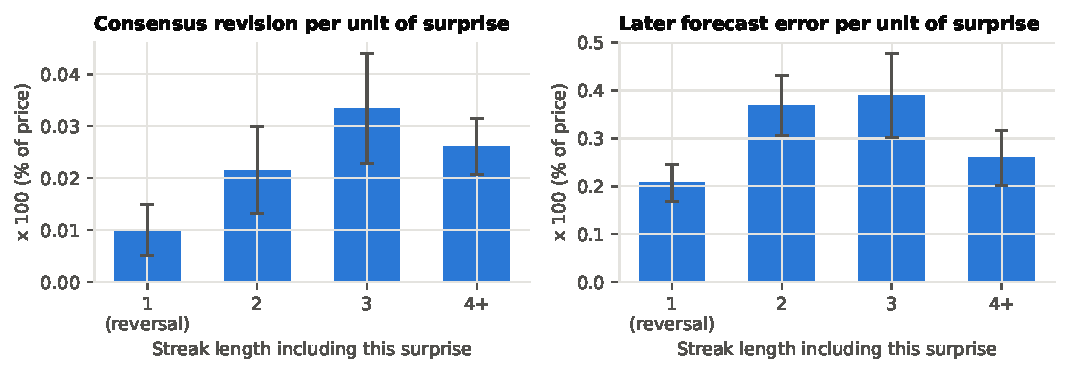
\includegraphics[width=0.97\textwidth]{results/fig_main.pdf}\end{center}

\begin{center}\small
\begin{tabular}{lccc}
\toprule
Slope on SUE (\% of price per unit) & Reversal & Extra for continuation & $t$ (extra)\\
\midrule
Consensus revision, SRW streaks & 0.010 & $+0.016$ & 4.9\\
Later forecast error, SRW streaks & 0.207 & $+0.101$ & 4.6\\
Later forecast error, XGBoost surprises and streaks & 0.149 & $+0.188$ & 8.6\\
\midrule
Price drift, months $+1..+3$ (all / covered / not covered) & 0.45 & $+0.13$ / $+0.17$ / $+0.00$ & 1.5 / 1.4 / 0.0\\
\bottomrule
\end{tabular}
\end{center}

\sect{Findings}
\begin{itemize}
\item \textbf{Analysts do not expect streaks to reverse.} The consensus moves \emph{more} per unit of surprise after a
  continuation, and more again with streak length (0.010 for reversals, 0.022--0.033 for streaks). That is the
  opposite of a naive gambler's fallacy.
\item \textbf{They still underreact more to streaks, mostly to short ones.} Even after revising, the consensus misses
  more of a streak surprise. The error slope is 0.21 after reversals, 0.37--0.39 after streaks of 2--3, and only 0.26
  after streaks of 4 or more. Underreacting to short streaks and catching up on long ones is what
  Rabin and Vayanos (2010) predict for believers in the fallacy. The pattern is stronger with XGBoost surprises
  ($t=8.6$), which are close to independent, so the streak carries less real information.
\item \textbf{The link to prices is inconclusive here.} In this simple specification the streak effect in the
  three-month price drift is positive but insignificant ($t=1.5$). It is present only in analyst-covered firms (0.17
  against 0.00), which fits analysts transmitting the bias, but it is too weak to test mediation.
\end{itemize}

\sect{Assessment and next steps}
Promising, and a natural mechanism section or companion paper for the gambler's-fallacy project. Analysts do
underweight short streaks, though not by expecting reversals. Next steps: (i) run the price test inside the
paper's own Fama--MacBeth framework and add analysts' forecast error as a mediator; (ii) get I/B/E/S detail data
(individual analysts and fiscal-year targets) for a clean forecast error and analyst-level fallacy measures, in the
spirit of Chen, Moskowitz and Shue (2016); (iii) separate up- and down-streaks, since optimism differs by sign.

{\footnotesize \textbf{References.} Rabin and Vayanos (2010, RES); Chen, Moskowitz and Shue (2016,
QJE); Loh and Warachka (2012, MS); Abarbanell and Bernard (1992, JF).}
\end{document}
